\subsection{Data Analysis}\label{sec:data-analysis}

This section presents relevant methods for analysing qualitative data and quantitative data.

\subsubsection{Analysing Qualitative Data}

Below, methods for analysing qualitative data are presented. In the research phase, Personas or Need groups are methods to analyse the though users of a product or a service. A Customer Journey Map supports understanding of how such users interact with a product or a service. Getting feedback from users involves getting ideas or suggestions for improvement of a product or a service. To analyse these, a sprint backlog is used to keep track of the priority of such feedback. If the features are then successfully implemented in the eyes of the users and stakeholders, can be tested using a sprint demo, where feedback is gathered for future work.

\subsubsection{Persona or Need groups}
When creating a product or a service, it is important to understand who you are designing for. Since the intended users might not always be around during the development phase, it helps having a clear mental image of the user. Fictional examples of users are one method to do this, either by using personas or need groups.

A \textit{persona} is a fictional character, created to give an example of the user who you are designing your service for \citep{stickdorn}. Depending on how broad the target group is for the service you are building, the persona might have several different needs. Then, dividing the though user groups in terms of designing for their different needs than their character traits might be more helpful \citep{expedition-mondial}. Dividing users by needs, if called forming \textit{need groups}. A need group (like "The beginner" or "The planner") can be described by their behaviour and their need.

Personas and need groups should be developed from research insights gathered from interviews or workshops with users and stakeholders \citep{stickdorn}.

\subsubsection{Customer Journey Map}
A customer journey map is said to provide a vivid but structured visualisation of a service user's experience \citep{stickdorn}. A typical customer journey is multi-channel and time-based, see figure \ref{cjmExample}

\begin{figure}[h]
    \centering
    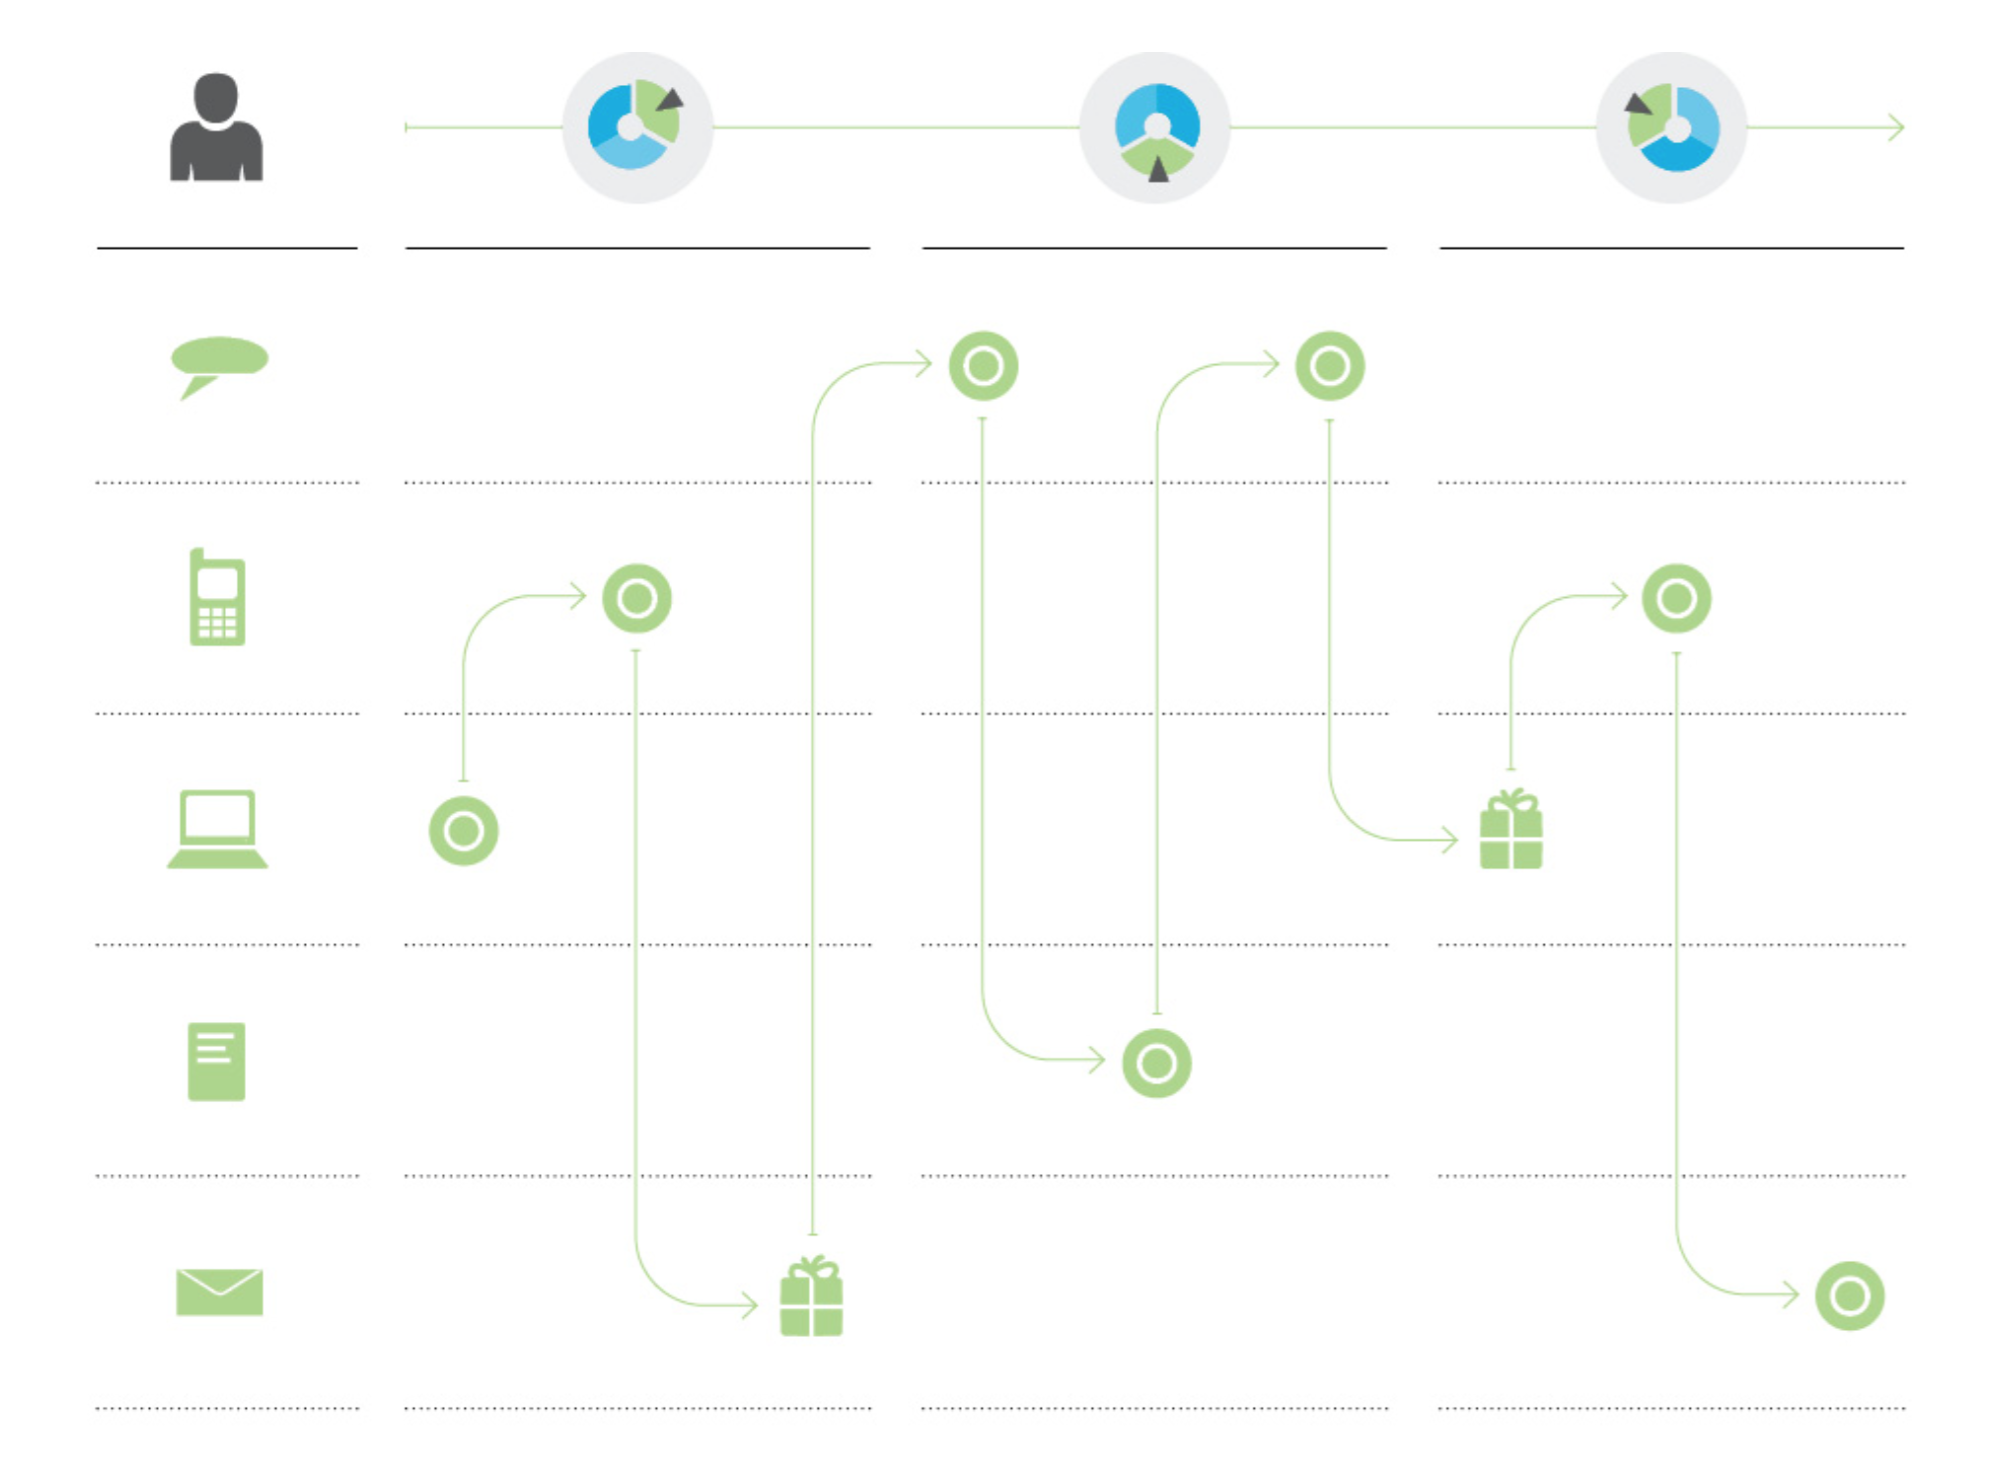
\includegraphics[width=0.7\textwidth]{analysis/cjmExample.png}
    \caption{General example of a customer service map. The map is divided by channel (could also be by a persona) and time (in this case before, during and after using a service).}
    \label{fig:cjmExample}
\end{figure}

The customer journey map is beneficial both for understanding a user's touchpoints with a service, and also for collecting and analysing stories which explain why the journeys happened as they did \citep{stickdorn}.

\subsubsection{Sprint Backlog}
During product development, to do a sprint backlog is a kind of data analysis. When a high altitude of ideas and feedback has been gathered, a sprint backlog is a list sorted with the most important and urgent items on top.

To work through ideas in a structured way, requests are categorized into what is called "stories". A good story answers "As a [user type] I want to be able to do [feature] so that [benefit]". Each story can then be broken down into todos ("What needs to be done in order to satisfy the story?"). During the sprint planning, the most important stories and todos are identified. By analysing and then working on the most prioritized story and todo, you ensure that you are always working on what is most important for the success of the project.

At the end of an iteration, as much as possible of the sprint backlog has been taken from "Not done" to "Done". The things not done, can either be moved into a product backlog (to later be added into an upcoming sprint backlog) or removed (they were not important enough).

\subsubsection{Sprint Demo}
A sprint demo is an effective way to analyse the product created after an iteration, from the perspective of the users and the stakeholders. \cite{kniberg} says that a well executed sprint demo attracts vital feedback from stakeholders, and ensures that todos are 100\% done. A sprint demo does not need to be complicated: the product is shown and tested with users and stakeholders, getting feedback for the next iteration. But without it, it would not be possible to know if the work done has satisfied the needs of the end users, or what the stakeholders thinks is important for future work. The sprint demo in this project is evaluated both with stakeholders and the end target group, the coaches. Evaluation is done by the interaction design principles: desirability (does the coach desire to use the product?), utility (does it meet the needs of the coach?), usability (is the coach able to use it without frustration?) and pleasurability (is the coach satisfied using the product?) \citep{lowgren}.

\subsubsection{Analysing Quantitative Data}
Below, methods for analysing collected quantitative data are presented. The first method used is correlation, but if multiple variables needs to taken into account, logistical regression can be used. As both of these are statistical tools, they rely on statistical significance in order to be trustworthy. In R programming language there are powerful tools for visualizing the correlation, for example using a "Correlation Heatmap", see figure \ref{fig:corrHeatmap}. In small-scale app tests, such amounts of data might not be sufficient.

To find trends or oddities in a small data set, visualization techniques to discover the quantitative data by hand might be more beneficial. To enable a visualization, data needs to be acquired, enhanced, mapped to a geometry and lastly rendered \citep{timo-ropinski-liu}. When rendered, a suitable rendering of a multiple-variable data set might be parallel coordinates, see figure \ref{fig:uneTerre}. Made interactive, each axis can be made filterable by user interaction.

\begin{figure}[h]
    \centering
    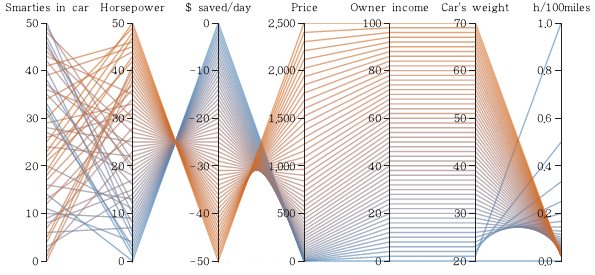
\includegraphics[width=0.7\textwidth]{analysis/terre.png}
    \caption{A parallel coordinates visualization enables you to visually observe relationships and trends between dimensions: positive or negative relationship (correlation or invert), or no relationship at all (random) \cite{une-terre}}
    \label{fig:uneTerre}
\end{figure}

%\subsubsection{Calculating Correlation in Google Sheets and R}

%The process is to calculate and compare means on a "control"  with a response variable.

%It is clear that analysis in Google Sheets can only go so far. It can be greatly helpful to sort by multiple columns (e.g. first by Manual?, then by School level, then by Quiz 3). However, it takes a long time to filter the data on multiple parameters, and the work easily becomes tedious. For some applications, it may not be viable to discover the data using this approach.

%In Google Sheets, color scale can be used to give different column values different colors, see figure \ref{analysFarg4}. It is still hard to compare all of the axises towards all the axises, and it is not a scientific approach.

%Even in R, it is cumbersome to do statistically with all of the axises against all the axises. It is however possible to in both Google Sheets as well as the R programming language. Psuedo-code in R would be:

%\begin{verbatim}
%x1 = c(1,2,3,1,5,6)
%x2 = c(2,3,4,NA,6,7)
%cor(x = x1, y = x2)
%cor.test(x1,x2)
%\end{verbatim}

%In R programming language there are powerful tools for visualizing the correlation, for example using a "Correlation Heatmap", see figure \ref{fig:corrHeatmap}. %Psuedo-code in R would be:

%\begin{verbatim}
%random_matrix <- matrix(rnorm(100), nrow = 10, ncol = 10)
%random_matrix[1,1] <- NA
%colnames(random_matrix) <- paste("V",1:10)
%cor_mat <- cor(random_matrix)
%heatmap(cor_mat, keep.dendro = FALSE)
%\end{verbatim}

\begin{figure}[h]
    \centering
    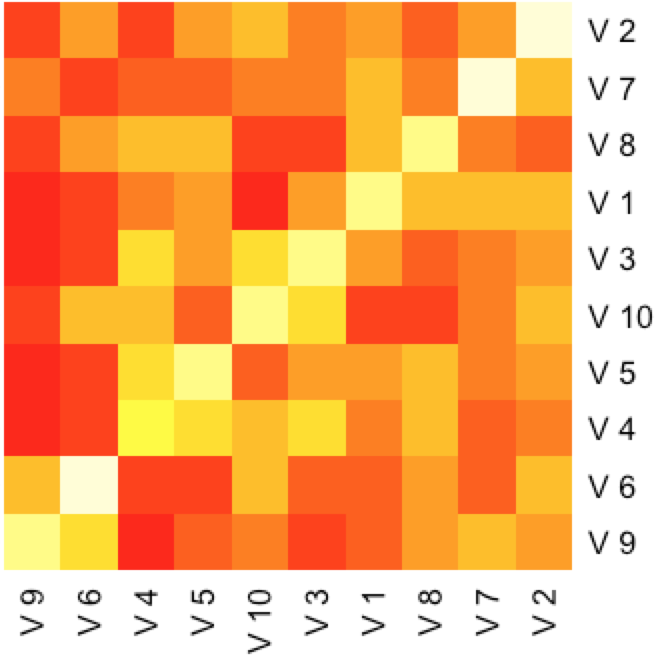
\includegraphics[width=0.7\textwidth]{analysis/rStatisticalAnalysis.png}
    \caption{Heatmap showing correlation, axis against axis, using example data. The more red a segment is, the bigger is the correlation between those two axises. You can see that in this example, there is a big correlation between for example V4 and V9. To be significantly significant in correlation or linear correlation, a common measure is that the Pr value ("the p-value") needs to be higher than 0.05. If the p-value is higher than 0.05, it means that it is significant with a 95\% probability.}
    \label{fig:corrHeatmap}
\end{figure}

%\subsubsection{Calculating Logistic Regression in R}

%A limitation with correlation is that only two dimensions can be compared with each other at the same time. What if we want to find a correlation between quiz score and gender \textit{and} age?

%To do this, Logistic Regression is helpful if our response variable can be a logistical dimension (e.g. women or male, used manual or not), while linear regression needs to be used if it is a linear or nominal scale (e.g. age and city respectively).

%In either case, the first step is to determine a response variable: the variable to compare against, e.g. is there a difference between men and women? In this case, it needs to be a quantitative measure of: "Have you learned anything?".

%If one more variable is added, e.g. also adding if a manual was used, this is called the "control". It is possible to add as many controls as possible.

%If linear regression, then it is needed to determine a quantitative measure of ("How much have you learned?").

%In Google Sheets, this is not effective to do. R, however, is a very suitable tool. First, the data is loaded, e.g. as a CSV file. Then, we tell R which the N/A values are, e.g. "N/A" or "Vet ej". We use this to filter the data. Then, each column we want to use is converted into a factor.

%When factors, a model can be created, e.g. using the General Linear Model. A different family can be selected, e.g. binomial.

%Then it is possible for R to show this data, showing the coefficient, the Pr value, and others. See code below.

%\begin{verbatim}
%mydata <- read.csv("Development/R/quizResults.csv", na.strings = c("N/A", "Vet ej"))

%mydata$y = ifelse(test = is.na(mydata$Quiz.9..y.n.1st),  yes = 0, no = 1)

%mydata$y <- as.factor(mydata$y)
%mydata$Help <- as.factor(mydata$Help)
%mydata$Sex <- as.factor(mydata$Sex)

%mymodel <- glm(formula = y ~ Pre.test.score + Sex, data = mydata, family = 'binomial')

%summary(mymodel)
%plot()

%\end{verbatim}

%For analysis, looking at the summary, coefficient (e.g. -1.0704) shows either a negative or positive correlation (in this case -7\%) for what to compare with as a response variable.

%To be significantly significant, a common measure is that the Pr value ("the p-value") needs to be higher than 0.05. If the p-value is higher than 0.05, it means that it is significant with a 95\% probability.

%\subsubsection{Visualizing and Analysing Multi-Variable Data with Parallel Coordinates}

%\cite{timo-ropinski-liu} describes the "visualization pipeline", generating an image from data:

%\begin{enumerate}
%\item Data acquisition ($\,\to\,$data are given)
%\item Data enhancement ($\,\to\,$ data are processed)
%\item Visualization mapping ($\,\to\,$ data are mapped to for example a geometry)
%\item Rendering ($\,\to\,$ images generated)
%\end{enumerate}

% Timo Ropinski, Scientific Visualization Group, Linköping University, TNM067 - Scientific Visualization, 9/12/2014)
% https://drive.google.com/drive/u/0/folders/0BzlK1PD8EE75bHIxcXRQNWpRMm8

%Data acquisition presents how data was acquired. Data enhancement explains how the data was processed. Visualization mapping is the process of mapping data to e.g. a geometry. Finally, rendering allows images to be generated, presented in 2D. This image can then be analysed.

%Parallel coordinates allows you to see relationships and trends between dimensions. They can be seen by a positive or negative relationship (correlation or invert), or no relationship at all (random) \cite{une-terre}. Parallel coordinates is not a quantitative data analysis per se, but it makes the data visually discoverable for visual analysis by a human. The human can more easily find patterns or outliers with a powerful visual representation.
